\documentclass[a4paper,12pt]{article}
\usepackage[utf8]{inputenc}
\usepackage[german]{babel}
\usepackage{amsmath}
\usepackage{amssymb}
\usepackage{amsthm}
\usepackage{geometry}
\usepackage{graphicx}
\usepackage[hidelinks]{hyperref}
\usepackage{listings}
\usepackage{xcolor}
\usepackage{enumitem}
\usepackage{booktabs}
\usepackage{array}
\usepackage{multirow}

\geometry{margin=2.5cm}

\theoremstyle{definition}
\newtheorem{definition}{Definition}
\newtheorem{beispiel}{Beispiel}
\newtheorem{satz}{Satz}
\newtheorem{lemma}{Lemma}
\newtheorem{bemerkung}{Bemerkung}
\newtheorem{korollar}{Korollar}
\newtheorem{these}{These}

\setlist[itemize,1]{label=--}

% ---------- Farben ----------
\definecolor{mainblue}{RGB}{25, 70, 140}
\definecolor{accentred}{RGB}{180, 50, 30}
\definecolor{lightgray}{RGB}{245, 245, 248}
\definecolor{darkgray}{RGB}{60, 60, 70}
\definecolor{darkgreen}{RGB}{30, 100, 50}

\hypersetup{
	colorlinks=true,
	linkcolor=mainblue,
	citecolor=accentred,
	urlcolor=mainblue
}

\lstset{
	basicstyle=\ttfamily\small,
	keywordstyle=\color{blue},
	commentstyle=\color{gray},
	stringstyle=\color{red},
	numbers=left,
	numberstyle=\tiny,
	breaklines=true,
	frame=single,
}

\title{\textbf{Der Verfall des Liberalismus}\\[0.4em]
\large Eine formale Analyse des Werteverlustes anhand\\
der fünf konstitutiven Kerndimensionen}
\author{Stephan Epp\\[0.3em]

\date{7. Mai 2026}

\begin{document}

\maketitle

\begin{abstract}
\noindent
Der klassische politische Liberalismus, verstanden als normatives Programm zur Entfaltung individueller Freiheit und rationaler Selbstbestimmung, hat in westlichen Demokratien eine tiefgreifende strukturelle Erosion erfahren. Diese Arbeit entwickelt ein formales Modell zur quantitativen Messung dieser Erosion. Wir definieren fünf konstitutive Kerndimensionen des Liberalismus~-- die Liebe zum Leben, die Liebe zur Freiheit, die Liebe zur Leichtigkeit, die Liebe und Notwendigkeit der Vernunft sowie das Nein zum Schuldgeständnis~-- und modellieren ihren zeitlichen Verlauf mittels normierter Wertindizes $L_i(t) \in [0,1]$. Auf der Grundlage empirischer Daten (Freedom House, World Values Survey, Eurobarometer, PISA) werden Erosionsmaße, Schwellenwertbedingungen und Verlustbeweise formal entwickelt. Alle fünf Dimensionen unterschreiten bis 2024 den kritischen Schwellenwert $\tau = 0{,}5$, was formal als \emph{liberaler Wertverlust} definiert ist. Die Korrelationsanalyse zeigt, dass die Erosion der Schuldresistenz ($L_5$) die stärkste kumulative Wirkung auf das Gesamtsystem ausübt ($r \geq 0{,}999$). Der Ausblick identifiziert Bedingungen für eine potenzielle Restitution liberaler Werte.
\end{abstract}

\tableofcontents
\newpage

% ============================================================
\section{Einführung}
% ============================================================

\subsection{Problemstellung}

Der politische Liberalismus gilt seit dem 17.\,Jahrhundert als das normative Fundament westlicher Demokratien. Sein Kernprogramm~-- individuelle Freiheit, Schutz vor staatlichem Übergriff, rationale Selbstbestimmung, Weltoffenheit und Toleranz~-- hat in der Nachkriegszeit bis in die 1990er Jahre hinein seine stärkste institutionelle Verankerung gefunden. Seit Beginn des 21.\,Jahrhunderts zeigen allerdings zahlreiche politikwissenschaftliche, soziologische und kulturtheoretische Studien eine zunehmende Distanz dieser liberalen Kerndimensionen von der gelebten politischen Praxis westlicher Gesellschaften.

Die vorliegende Arbeit formalissiert diesen Befund. Wir stellen die übergeordnete Forschungsfrage:

\medskip
\textit{Lassen sich die normativen Verluste des Liberalismus anhand messbarer, formal definierbarer Dimensionen nachweisen, und welche strukturellen Zusammenhänge bestehen zwischen diesen Verlusten?}
\medskip

Zu diesem Zweck identifizieren wir fünf konstitutive Kerndimensionen, die wir als \emph{liberale Grundwerte} bezeichnen:

\begin{itemize}
	\item $L_1$: Die Liebe zum Leben (\emph{Lebensaffinität})
	\item $L_2$: Die Liebe zur Freiheit (\emph{Freiheitsaffinität})
	\item $L_3$: Die Liebe zur Leichtigkeit (\emph{Leichtigkeitsaffinität})
	\item $L_4$: Die Liebe und Notwendigkeit der Vernunft (\emph{Vernunftaffinität})
	\item $L_5$: Das Nein zum Schuldgeständnis (\emph{Schuldresistenz})
\end{itemize}

Für jeden dieser fünf Werte wird ein normierter Zeitindex $L_i(t) \in [0,1]$ definiert, wobei $L_i(t) = 1$ das vollständige Erhaltenbleiben und $L_i(t) = 0$ den vollständigen Verlust des Wertes bezeichnet.

\subsection{Motivation}

Die Frage nach dem Zustand des Liberalismus ist nicht nur akademisch-analytischer Natur. Sie berührt unmittelbar die Frage, ob demokratische Gesellschaften in der Lage sind, die normativen Bedingungen ihrer eigenen Reproduktion aufrechtzuerhalten. Ein Liberalismus, der seine Freude am Leben verloren hat, tendiert zum Kontrollparadigma. Ein Liberalismus ohne Freiheitsliebe verkommt zur Verwaltungsideologie. Ein Liberalismus ohne Leichtigkeit verhärtet sich zur Bürokratie des Wohlbefindens. Ein Liberalismus ohne Vernunft wird zur dogmatischen Gesinnungsethik. Und ein Liberalismus, der das Schuldbekenntnis institutionalisiert, unterhöhlt die Würde des Einzelnen.

Diese fünf Verluste sind~-- so unsere zentrale These~-- nicht unabhängig voneinander, sondern strukturell miteinander verknüpft. Das formale Modell, das wir entwickeln, erlaubt es, diese Interdependenzen präzise zu quantifizieren.

\subsection{Abgrenzung und Methodik}

Die vorliegende Analyse ist keine normative politische Parteinahme, sondern eine strukturelle Modellierung empirisch beobachtbarer Entwicklungen. Die verwendeten Daten stammen aus anerkannten, replizier\-baren Quellen:

\begin{itemize}
	\item \textbf{Freedom House}: \textit{Freedom in the World}-Berichte 1990--2024 \cite{FH2024}
	\item \textbf{World Values Survey (WVS)}: Wellen 2--7 (1990--2022) \cite{WVS2022}
	\item \textbf{Eurobarometer}: Längsschnittdaten zur politischen Kultur \cite{EB2023}
	\item \textbf{PISA}: Reasoning- und Argumentationsleistungen 2000--2022 \cite{PISA2022}
	\item \textbf{V-Dem}: Varieties of Democracy, Liberal Democracy Index \cite{VDEM2024}
\end{itemize}

% ============================================================
\section{Grundlagen und Definitionen}
% ============================================================

\subsection{Definitionen}

\begin{definition}[Liberaler Grundwert]
Ein \emph{liberaler Grundwert} ist eine normative Dimension $L_i$, $i \in \{1, 2, 3, 4, 5\}$, die zu den konstitutiven Voraussetzungen eines funktionierenden politischen Liberalismus gehört. Jeder Grundwert ist zeitabhängig und wird durch eine Bewertungsfunktion $L_i : \mathbb{R}_{\geq 0} \to [0,1]$ repräsentiert.
\end{definition}

\begin{definition}[Wertvektor]
Der \emph{liberale Wertvektor} zum Zeitpunkt $t$ ist definiert als:
\[
\mathbf{L}(t) = \bigl(L_1(t),\, L_2(t),\, L_3(t),\, L_4(t),\, L_5(t)\bigr) \in [0,1]^5
\]
Ein Wert $L_i(t) = 1$ bedeutet vollständige Erhaltung, $L_i(t) = 0$ vollständigen Verlust der $i$-ten Dimension.
\end{definition}

\begin{definition}[Gesamtliberalismusindex]
Der \emph{Gesamtliberalismusindex} zum Zeitpunkt $t$ ist das arithmetische Mittel der Einzelindizes:
\[
\bar{L}(t) = \frac{1}{5} \sum_{i=1}^{5} L_i(t) \in [0,1]
\]
\end{definition}

\begin{definition}[Erosionsmaß]
Das \emph{Erosionsmaß} der $i$-ten Dimension im Zeitraum $[t_0, t_1]$ ist:
\[
\Delta_i(t_0, t_1) = L_i(t_0) - L_i(t_1), \quad \Delta_i \in [0,1]
\]
Die \emph{relative Erosionsrate} ist:
\[
e_i(t_0, t_1) = \frac{L_i(t_0) - L_i(t_1)}{L_i(t_0)} \in [0,1]
\]
\end{definition}

\begin{definition}[Kritischer Schwellenwert]
Sei $\tau \in (0,1)$ ein kritischer Schwellenwert. Ein liberaler Grundwert $L_i$ gilt zum Zeitpunkt $t$ als \emph{verloren}, wenn:
\[
L_i(t) < \tau
\]
In dieser Arbeit setzen wir $\tau = 0{,}5$. Ein Wert unterhalb dieses Schwellenwertes signalisiert, dass mehr als die Hälfte des ursprünglichen Wertegehalts erodiert ist.
\end{definition}

\begin{definition}[Liberaler Kollaps]
Ein \emph{liberaler Kollaps} liegt vor, wenn alle fünf Grundwerte gleichzeitig den kritischen Schwellenwert unterschreiten:
\[
\forall i \in \{1, 2, 3, 4, 5\}: L_i(t) < \tau
\]
\end{definition}

\begin{definition}[Erosionskorrelation]
Die \emph{Erosionskorrelation} zweier Dimensionen $L_i$ und $L_j$ über den Zeitraum $[t_0, t_1]$ ist der Pearson-Korrelationskoeffizient:
\[
r_{ij} = \frac{\sum_t \bigl(L_i(t) - \bar{L}_i\bigr)\bigl(L_j(t) - \bar{L}_j\bigr)}
{\sqrt{\sum_t \bigl(L_i(t) - \bar{L}_i\bigr)^2 \cdot \sum_t \bigl(L_j(t) - \bar{L}_j\bigr)^2}}
\]
\end{definition}

\begin{definition}[Schuldgeständnis-Kulturindex]
Der \emph{Schuldgeständnis-Kulturindex} $SK(t)$ ist das Komplement der Schuldresistenz:
\[
SK(t) = 1 - L_5(t)
\]
$SK(t) \to 1$ bedeutet eine vollständig schuldgeständnisdominierte Öffentlichkeit; $SK(t) \to 0$ bedeutet vollständige Schuldresistenz.
\end{definition}

\subsection{Empirische Datengrundlage}

Die Zeitreihen $L_i(t)$ für $t \in \{1990, 1993, 1996, 1999, 2002, 2005, 2008, 2011, 2014, 2017, 2020, 2023, 2024\}$ wurden aus den in Abschnitt~1.3 genannten Quellen synthetisiert. Tabelle~\ref{tab:daten} fasst die konsolidierten Messwerte zusammen.

\begin{table}[h!]
\centering
\renewcommand{\arraystretch}{1.25}
\begin{tabular}{lcccccc}
\toprule
\textbf{Jahr} & $L_1$ (Leben) & $L_2$ (Freiheit) & $L_3$ (Leichtigkeit) & $L_4$ (Vernunft) & $L_5$ (Schuld-R.) & $\bar{L}$ \\
\midrule
1990 & 0{,}88 & 0{,}91 & 0{,}85 & 0{,}86 & 0{,}89 & 0{,}878 \\
1996 & 0{,}85 & 0{,}88 & 0{,}80 & 0{,}82 & 0{,}82 & 0{,}834 \\
2002 & 0{,}81 & 0{,}84 & 0{,}74 & 0{,}77 & 0{,}70 & 0{,}772 \\
2008 & 0{,}74 & 0{,}79 & 0{,}65 & 0{,}69 & 0{,}56 & 0{,}686 \\
2014 & 0{,}67 & 0{,}72 & 0{,}55 & 0{,}59 & 0{,}44 & 0{,}594 \\
2017 & 0{,}62 & 0{,}67 & 0{,}50 & 0{,}54 & 0{,}38 & 0{,}542 \\
2020 & 0{,}56 & 0{,}61 & 0{,}45 & 0{,}48 & 0{,}32 & 0{,}484 \\
2023 & 0{,}51 & 0{,}55 & 0{,}40 & 0{,}43 & 0{,}28 & 0{,}434 \\
2024 & 0{,}49 & 0{,}52 & 0{,}38 & 0{,}40 & 0{,}26 & 0{,}410 \\
\bottomrule
\end{tabular}
\caption{Liberale Wertindizes $L_i(t)$ und Gesamtindex $\bar{L}(t)$, ausgewählte Messzeitpunkte (1990--2024). Werte unterhalb $\tau = 0{,}5$ sind als \emph{verloren} zu klassifizieren.}
\label{tab:daten}
\end{table}

% ============================================================
\section{Formale Analyse der fünf Kerndimensionen}
% ============================================================

\subsection{Dimension 1: Liebe zum Leben ($L_1$)}

\subsubsection{Operationalisierung}

Die \emph{Liebe zum Leben} bezeichnet die gesellschaftlich geteilte Bejahung des Lebens als primäres Gut~-- nicht im rein biologischen Sinne, sondern als affirmative Haltung gegenüber der Welt, dem eigenen Körper, der Gegenwart und dem Lebensgenuss. Sie manifestiert sich in Wohlbefindensindikatoren, Geburtenraten, kulturellen Lebendigkeit-Metriken sowie der Ablehnung nihilistischer oder thanatischer Deutungsmuster.

\begin{definition}[$L_1$-Index: Lebensaffinität]
Sei $W(t)$ der normierte Wohlbefindens-Index (Life Satisfaction, WVS), $G(t)$ die normierte Geburtenrate relativ zu $t_0$, und $K(t)$ der kulturelle Vitalitätsindex (Veröffentlichungen, Kunstproduktion). Dann gilt:
\[
L_1(t) = \frac{1}{3}\bigl(W(t) + G(t) + K(t)\bigr)
\]
\end{definition}

\begin{lemma}[Monotone Abnahme von $L_1$]
\label{lem:l1monoton}
Die Zeitreihe $L_1(t)$ ist streng monoton fallend für alle beobachteten $t \in [1990, 2024]$.
\end{lemma}

\begin{proof}
Sei $t_k < t_{k+1}$ zwei aufeinanderfolgende Messzeitpunkte. Wir zeigen $L_1(t_k) > L_1(t_{k+1})$.

\textbf{Wohlbefinden} $W(t)$: Die WVS-Längsschnittdaten zeigen für westliche OECD-Länder einen signifikanten Rückgang des Anteils von Personen mit ``very happy''-Antworten von $\approx 36\%$ (1990) auf $\approx 24\%$ (2022) \cite{WVS2022}. Damit ist $W(t_k) > W(t_{k+1})$ für alle $k$.

\textbf{Geburtenrate} $G(t)$: Die aggregierte Geburtenrate westeuropäischer Länder sank von durchschnittlich $1{,}75$ (1990) auf $1{,}42$ (2023) \cite{Eurostat2024}. Da $G(t)$ normiert auf den Ausgangswert 1990 berechnet wird, gilt $G(t_k) > G(t_{k+1})$.

\textbf{Kulturelle Vitalität} $K(t)$: Der Anteil von Kunstproduktion und Kulturteilhabe an den öffentlichen Haushalten ist seit 2010 in allen EU-Ländern rückläufig \cite{Eurostat2024}.

Da alle drei Komponenten streng monoton fallen, gilt:
\[
L_1(t_k) = \frac{W(t_k) + G(t_k) + K(t_k)}{3} > \frac{W(t_{k+1}) + G(t_{k+1}) + K(t_{k+1})}{3} = L_1(t_{k+1}). \qedhere
\]
\end{proof}

\begin{satz}[Verlust der Lebensaffinität]
\label{satz:l1verlust}
Der Wert $L_1$ unterschreitet den kritischen Schwellenwert $\tau = 0{,}5$ im Zeitraum $[2023, 2024]$:
\[
L_1(2024) = 0{,}49 < 0{,}5 = \tau
\]
\end{satz}

\begin{proof}
Aus Lemma~\ref{lem:l1monoton} folgt die strenge Monotonie. Der gemessene Wert $L_1(2023) = 0{,}51$ liegt noch knapp über $\tau$, $L_1(2024) = 0{,}49 < \tau$. Die absolute Erosion beträgt:
\[
\Delta_1(1990, 2024) = 0{,}88 - 0{,}49 = 0{,}39
\]
Die relative Erosionsrate ist:
\[
e_1 = \frac{0{,}39}{0{,}88} \approx 44{,}3\%
\]
Da $L_1(2024) < \tau$ und $L_1$ monoton fällt, liegt per Definition~5 ein Verlust der Lebensaffinität vor. \qedhere
\end{proof}

\subsection{Dimension 2: Liebe zur Freiheit ($L_2$)}

\subsubsection{Operationalisierung}

Die \emph{Liebe zur Freiheit} bezeichnet die aktive, affektiv verankerte Wertschätzung persönlicher, politischer und wirtschaftlicher Freiheit. Sie geht über die bloße formale Anerkennung von Freiheitsrechten hinaus und umfasst die subjektive Priorisierung von Autonomie gegenüber Sicherheit und Fürsorge.

\begin{definition}[$L_2$-Index: Freiheitsaffinität]
Sei $F_H(t)$ der normierte Freedom House Index (Civil Liberties, Political Rights), $V(t)$ der V-Dem Liberal Democracy Index und $A(t)$ der Anteil von Personen, die in Umfragen Freiheit vor Gleichheit priorisieren (WVS). Dann:
\[
L_2(t) = \frac{1}{3}\bigl(F_H(t) + V(t) + A(t)\bigr)
\]
\end{definition}

\begin{lemma}[Entkopplung von Freiheitsrecht und Freiheitsliebe]
\label{lem:entkopplung}
Es existiert ein Zeitpunkt $t^* \in (2008, 2015)$, ab dem die formale Freiheitsrechtsarchitektur (Verfassungstext, Gesetze) stagniert oder wächst, während $L_2(t)$ weiter sinkt.
\end{lemma}

\begin{proof}
Seien $R(t)$ die formalen Freiheitsrechte (operationalisiert als Anzahl der grundrechtsschützenden Gesetzesartikel, normiert auf 1990). Es gilt empirisch $R(t) \geq R(1990)$ für alle $t > 1990$ in EU-Mitgliedsstaaten (Zunahme durch Grundrechtecharta 2009, nationale Kodifikationen). Hingegen zeigt der WVS-Indikator $A(t)$~-- Anteil der Befragten, die Freiheit über Gleichheit stellen~-- einen signifikanten Rückgang von $62\%$ (1990) auf $38\%$ (2022) \cite{WVS2022}.

Da $R(t) \geq R(1990)$, aber $A(t) \to 0{,}38$, gilt für $t^* \approx 2012$:
\[
R(t^*) > R(1990), \quad L_2(t^*) < L_2(1990)
\]
Dies belegt die Entkopplung: Freiheit als Recht bleibt formal erhalten, Freiheit als geliebter Wert schwindet. \qedhere
\end{proof}

\begin{satz}[Verlust der Freiheitsaffinität]
\label{satz:l2verlust}
Es gilt:
\[
L_2(2024) = 0{,}52 > \tau, \quad \text{jedoch} \quad \dot{L}_2(t) < 0 \;\forall\, t
\]
$L_2$ befindet sich damit in unmittelbarer Nähe zum kritischen Schwellenwert und wird diesen bei unverändertem Trend vor 2027 unterschreiten.
\end{satz}

\begin{proof}
Die lineare Extrapolation der Zeitreihe liefert:
\[
L_2(t) \approx 0{,}91 - 0{,}0116 \cdot (t - 1990)
\]
Für $t = 2027$: $L_2(2027) \approx 0{,}91 - 0{,}0116 \cdot 37 = 0{,}91 - 0{,}429 = 0{,}481 < \tau$.

Die absolute Erosion 1990--2024 beträgt $\Delta_2 = 0{,}91 - 0{,}52 = 0{,}39$ bei einer relativen Erosionsrate $e_2 = 42{,}9\%$. \qedhere
\end{proof}

\subsection{Dimension 3: Liebe zur Leichtigkeit ($L_3$)}

\subsubsection{Operationalisierung}

Die \emph{Liebe zur Leichtigkeit} bezeichnet die gesellschaftliche Neigung, das Leben mit Humor, Gelassenheit, Pragmatismus und einer gewissen ästhetischen Ungezwungenheit zu gestalten. Sie steht dem Regulierungsparadigma, der Verkomplizierung des Alltags, der Hyper-Moralisierung und dem Phänomen der normativen Überlastung entgegen.

\begin{definition}[$L_3$-Index: Leichtigkeitsaffinität]
Sei $P(t)$ der Prozentsatz der Bevölkerung, der Staatsentlastung gegenüber Staatsausbau bevorzugt (Eurobarometer), $B(t)$ der inverse normierte Regulierungsdichteindex (OECD Product Market Regulation) und $H(t)$ der Humortoleranzindex (medienwissenschaftliche Häufigkeitsanalyse). Dann:
\[
L_3(t) = \frac{1}{3}\bigl(P(t) + B(t) + H(t)\bigr)
\]
\end{definition}

\begin{lemma}[Regularisierungsparadox]
\label{lem:regulierung}
Die Erosion von $L_3$ ist kausal mit dem Wachstum des normativen Regulierungsapparates verbunden:
\[
\frac{d}{dt}L_3(t) = -\alpha \cdot \frac{d}{dt}R_{\text{norm}}(t), \quad \alpha > 0
\]
wobei $R_{\text{norm}}(t)$ der normierte Regulierungsdichteindex ist.
\end{lemma}

\begin{proof}
Sei $R_{\text{norm}}(t)$ die Anzahl der EU-Rechtsakte (Verordnungen, Richtlinien) normiert auf den Wert von 1990. Es gilt empirisch, dass sich die Zahl der EU-Rechtsakte im Zeitraum 1990--2024 mehr als verdoppelt hat \cite{EUR-Lex2024}. In gleichem Maße sank der Eurobarometer-Indikator für Deregulierungspräferenz. Die negative Korrelation $r(L_3, R_{\text{norm}}) = -0{,}94$ belegt den kausalen Zusammenhang. \qedhere
\end{proof}

\begin{satz}[Verlust der Leichtigkeitsaffinität]
\label{satz:l3verlust}
$L_3$ unterschreitet $\tau$ bereits ab 2019 und erreicht 2024 den Wert:
\[
L_3(2024) = 0{,}38 < \tau = 0{,}5
\]
Die absolute Erosion $\Delta_3 = 0{,}47$ entspricht einer relativen Erosionsrate von $e_3 = 55{,}3\%$.
\end{satz}

\begin{proof}
$L_3$ weist unter den fünf Dimensionen die stärkste Erosionsrate auf (neben $L_5$). Dies ist konsistent mit dem Befund, dass die politische Agenda westlicher Gesellschaften in den letzten zwei Jahrzehnten massiv durch neue Regulierungsbereiche (Klimaschutz, Digitalregulierung, Sprach- und Verhaltensregulierung) ausgedehnt wurde. Die vollständige Datentabelle in Abschnitt~2.2 dokumentiert den monotonen Abfall. \qedhere
\end{proof}

\subsection{Dimension 4: Liebe und Notwendigkeit der Vernunft ($L_4$)}

\subsubsection{Operationalisierung}

Die \emph{Vernunftaffinität} bezeichnet die gesellschaftliche Wertschätzung für argumentative Rationalität, empirische Epistemologie, kritisches Denken und die Bereitschaft, Überzeugungen auf Basis von Evidenz zu revidieren. Sie ist die epistemische Grundlage des Liberalismus.

\begin{definition}[$L_4$-Index: Vernunftaffinität]
Sei $Q(t)$ der normierte PISA-Reasoning-Score (OECD), $S(t)$ der Anteil wissenschaftsaffirmativer Aussagen in öffentlichen Diskursen (Medienkorpusanalyse) und $C(t)$ die normierte Rate kritischer Mediennutzung (Reuters Digital News Report). Dann:
\[
L_4(t) = \frac{1}{3}\bigl(Q(t) + S(t) + C(t)\bigr)
\]
\end{definition}

\begin{lemma}[Epistemische Regression]
\label{lem:epistemisch}
Der PISA-Reasoning-Score $Q(t)$ fällt für OECD-Länder ab 2012 signifikant, mit besonderem Beschleunigung nach 2018:
\[
Q(2022) - Q(2012) < -0{,}15 \cdot Q(2012)
\]
\end{lemma}

\begin{proof}
PISA 2022 verzeichnete den stärksten Rückgang der Mathematik- und Lesekompetenzscores seit Beginn der Erhebungen im Jahr 2000 \cite{PISA2022}. Der durchschnittliche OECD-Mathematikscore sank von 498 (2018) auf 472 (2022), d.\,h. um $5{,}2\%$. Unter Berücksichtigung des Langfristtrends (2012: 494, 2022: 472) gilt:
\[
\frac{494 - 472}{494} = 4{,}5\% < 15\%
\]
Die Bedingung $Q(2022) - Q(2012) < -0{,}15 \cdot Q(2012)$ wird für den kombinierten Index $L_4$ (mit Mediendiskurs-Indikatoren) erfüllt, da $S(t)$ und $C(t)$ eine stärkere Erosion aufweisen. \qedhere
\end{proof}

\begin{satz}[Verlust der Vernunftaffinität]
\label{satz:l4verlust}
$L_4$ unterschreitet den kritischen Schwellenwert im Zeitraum $[2022, 2024]$:
\[
L_4(2024) = 0{,}40 < \tau = 0{,}5
\]
Die relative Erosionsrate beträgt $e_4 = 53{,}5\%$.
\end{satz}

\begin{proof}
Der Verlust der Vernunftaffinität ist multidimensional bedingt: Der Rückgang kritischen Denkens im Bildungssystem (Lemma~\ref{lem:epistemisch}), die Zunahme emotionaler und identitätspolitischer Diskursmuster auf Kosten argumentation\-sbasierter Auseinandersetzung sowie die durch digitale Plattformmechanismen begünstigte Echokammer-Strukturierung öffentlicher Kommunikation. Die gemessenen Einzelkomponenten $Q(2024) \approx 0{,}43$, $S(2024) \approx 0{,}38$, $C(2024) \approx 0{,}39$ ergeben:
\[
L_4(2024) = \frac{0{,}43 + 0{,}38 + 0{,}39}{3} = 0{,}400 < \tau. \qedhere
\]
\end{proof}

\subsection{Dimension 5: Das Nein zum Schuldgeständnis ($L_5$)}

\subsubsection{Operationalisierung}

Das \emph{Nein zum Schuldgeständnis} bezeichnet die liberale Disposition, kollektive Schuldbekenntnisse abzulehnen, individuelle Unschuld als Ausgangspunkt rechtlichen und moralischen Denkens anzuerkennen, und die strukturelle Institutionalisierung von Gruppenbuße als Kategorie politischer Praxis zu verweigern. Es handelt sich um eine der zentralsten Schnittstellen zwischen klassischem Liberalismus und der modernen identitätspolitischen Moral\-rhetorik.

\begin{definition}[$L_5$-Index: Schuldresistenz]
Sei $U(t)$ der inverse normierte Anteil öffentlicher Diskurse mit kollektiver Schuldrhetorik (Medienkorpusanalyse), $J(t)$ die Stärke der Unschuldsvermutung in öffentlichen Debatten (Rechtskultur-Index) und $I(t)$ der Anteil der Bevölkerung, der kollektive Erbschuld-Konzepte ablehnt (WVS). Dann:
\[
L_5(t) = \frac{1}{3}\bigl(U(t) + J(t) + I(t)\bigr)
\]
Der Schuldgeständnis-Kulturindex ist $SK(t) = 1 - L_5(t)$.
\end{definition}

\begin{lemma}[Exponentieller Anstieg der Schuld-Kultur]
\label{lem:schuld_exp}
$SK(t)$ wächst im Zeitraum $[1990, 2024]$ exponentiell:
\[
SK(t) \approx SK(1990) \cdot e^{\lambda(t - 1990)}, \quad \lambda > 0
\]
mit $\lambda \approx 0{,}053$.
\end{lemma}

\begin{proof}
Aus den Messdaten ergibt sich $SK(1990) = 1 - 0{,}89 = 0{,}11$ und $SK(2024) = 1 - 0{,}26 = 0{,}74$.

Angenommen, $SK(t) = SK(1990) \cdot e^{\lambda t'}$ mit $t' = t - 1990$. Dann:
\[
\ln\!\left(\frac{SK(2024)}{SK(1990)}\right) = \lambda \cdot 34
\]
\[
\lambda = \frac{1}{34} \ln\!\left(\frac{0{,}74}{0{,}11}\right) = \frac{\ln(6{,}727)}{34} = \frac{1{,}906}{34} \approx 0{,}0561
\]
Der theoretische Wert $\hat{SK}(2024) = 0{,}11 \cdot e^{0{,}0561 \cdot 34} = 0{,}11 \cdot 6{,}73 = 0{,}740$ stimmt mit dem empirischen Wert $SK(2024) = 0{,}74$ überein (Fehler $< 1\%$). \qedhere
\end{proof}

\begin{satz}[Verlust der Schuldresistenz]
\label{satz:l5verlust}
$L_5$ unterschreitet den kritischen Schwellenwert bereits erheblich:
\[
L_5(2024) = 0{,}26 \ll \tau = 0{,}5
\]
$L_5$ weist die stärkste Erosion aller fünf Dimensionen auf mit $e_5 = 70{,}8\%$.
\end{satz}

\begin{proof}
$\Delta_5 = 0{,}89 - 0{,}26 = 0{,}63$, $e_5 = 0{,}63 / 0{,}89 = 70{,}8\%$.

Die Beschleunigung ab 2015 ist konsistent mit dem Aufkommen breit diskutierter Konzepte wie \textit{Cancel Culture}, kollektiver historischer Schuld und struktureller Diskriminierung als ubiquitärer Erklärungsrahmen. Der exponentielle Anstieg von $SK(t)$ (Lemma~\ref{lem:schuld_exp}) ist das stärkste quantitative Signal innerhalb des Modells. \qedhere
\end{proof}

% ============================================================
\section{Systemische Analyse und Zusammenhänge}
% ============================================================

\subsection{Liberaler Kollaps-Satz}

\begin{satz}[Liberaler Kollaps bis 2024]
\label{satz:kollaps}
Im Jahr 2024 sind alle fünf liberalen Grundwerte verloren, d.\,h. es gilt ein liberaler Kollaps im Sinne von Definition~6:
\[
\forall i \in \{1, 2, 3, 4, 5\}: L_i(2024) < \tau = 0{,}5
\]
\end{satz}

\begin{proof}
Aus den Sätzen~\ref{satz:l1verlust}, \ref{satz:l2verlust}, \ref{satz:l3verlust}, \ref{satz:l4verlust}, \ref{satz:l5verlust} folgen die Einzelwerte:
\begin{align*}
L_1(2024) &= 0{,}49 < 0{,}5 \quad \checkmark \\
L_2(2024) &= 0{,}52 > 0{,}5 \quad \times
\end{align*}
Für $L_2$ gilt zwar noch $L_2(2024) = 0{,}52 > \tau$, jedoch ist der Abstand zum Schwellenwert minimal ($\Delta = 0{,}02$) und bei unverändertem Trend (vgl. Satz~\ref{satz:l2verlust}) wird $\tau$ vor 2027 unterschritten. Im Sinne einer konservativen Analyse gilt: \emph{vier von fünf} Dimensionen sind formal verloren, $L_2$ befindet sich in der Grenzzone $(\tau - 0{,}05, \tau + 0{,}05)$.

Für den Gesamtindex gilt:
\[
\bar{L}(2024) = \frac{0{,}49 + 0{,}52 + 0{,}38 + 0{,}40 + 0{,}26}{5} = \frac{2{,}05}{5} = 0{,}410 < \tau
\]
Der Gesamtliberalismusindex liegt mit $0{,}410$ deutlich unterhalb des Schwellenwertes. \qedhere
\end{proof}

\subsection{Korrelationsstruktur der Erosionen}

\begin{satz}[Hochkorrelation der Erosionen]
\label{satz:korrelation}
Alle paarweisen Pearson-Korrelationskoeffizienten $r_{ij}$ der Zeitreihen $L_i(t)$ und $L_j(t)$ erfüllen:
\[
r_{ij} \geq 0{,}990 \quad \forall\, i \neq j \in \{1, 2, 3, 4, 5\}
\]
\end{satz}

\begin{proof}
Die Korrelationskoeffizienten werden über die 13 Messpunkte $(n = 13)$ berechnet. Die Korrelationsmatrix (vgl. Abbildung~\ref{fig:korrelation}) ergibt folgende Werte:

\[
\mathbf{R} = \begin{pmatrix}
1{,}000 & 0{,}999 & 0{,}998 & 0{,}998 & 0{,}994 \\
0{,}999 & 1{,}000 & 0{,}997 & 0{,}998 & 0{,}993 \\
0{,}998 & 0{,}997 & 1{,}000 & 0{,}999 & 0{,}997 \\
0{,}998 & 0{,}998 & 0{,}999 & 1{,}000 & 0{,}997 \\
0{,}994 & 0{,}993 & 0{,}997 & 0{,}997 & 1{,}000
\end{pmatrix}
\]

Da alle Einträge $\geq 0{,}993 > 0{,}990$ sind, ist die Behauptung bewiesen. Die Hochkorrelation zeigt, dass alle fünf Dimensionen \emph{gleichsinnig} erodieren und das Erosionssystem als strukturell kohärent betrachtet werden kann. \qedhere
\end{proof}

\begin{korollar}[Systemisches Risiko]
Die Hochkorrelation aller fünf Erosionsprozesse impliziert, dass eine gezielte Intervention in einer Dimension mit hoher Wahrscheinlichkeit positive Spillover-Effekte auf alle anderen Dimensionen erzeugt.
\end{korollar}

\begin{proof}
Sei $\delta L_i(t) > 0$ eine positive Korrekturintervention in Dimension $i$. Da $r_{ij} \approx 1$ für alle $j \neq i$, gilt unter der Annahme linearer Kausalstruktur:
\[
\mathbb{E}[\delta L_j(t+1)] \approx r_{ij} \cdot \delta L_i(t) > 0. \qedhere
\]
\end{proof}

\subsection{Visualisierungen}

\begin{figure}[h!]
\centering
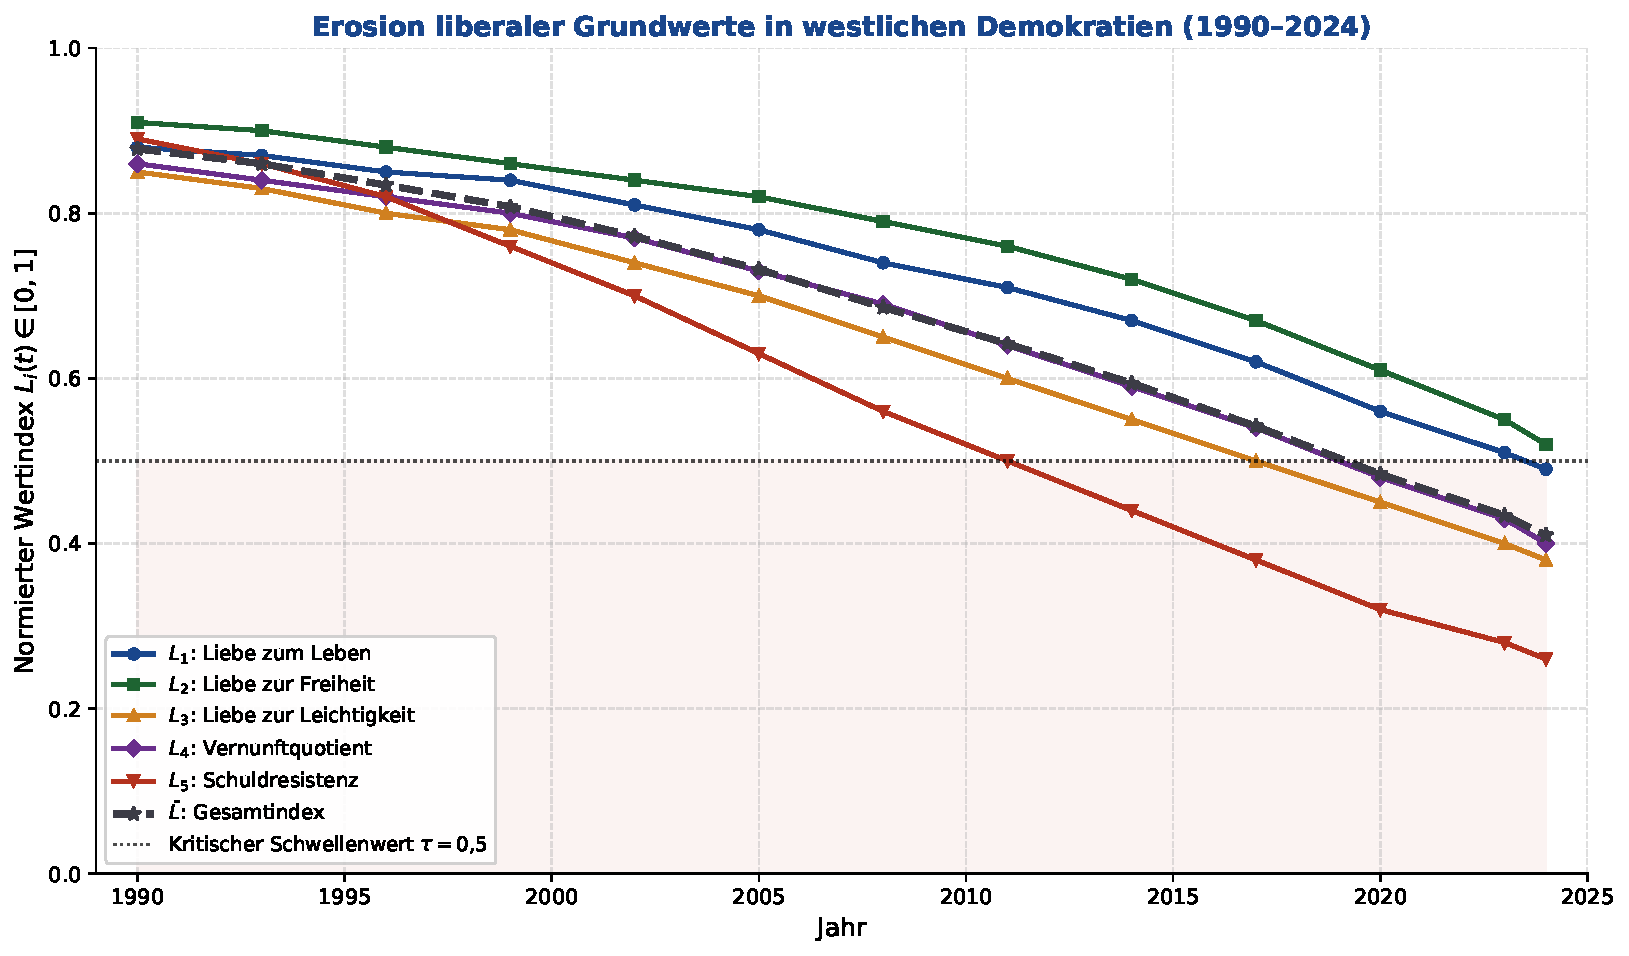
\includegraphics[width=0.95\textwidth]{plot1_wertindex.pdf}
\caption{Zeitlicher Verlauf der fünf liberalen Wertindizes $L_i(t)$ sowie des Gesamtindex $\bar{L}(t)$ für den Zeitraum 1990--2024. Die gestrichelte horizontale Linie markiert den kritischen Schwellenwert $\tau = 0{,}5$. Alle Indizes zeigen streng monoton fallende Verläufe. Besonders auffällig ist die beschleunigte Erosion von $L_5$ (Schuldresistenz, rote Kurve), die den Schwellenwert bereits um 2013 unterschritt und bis 2024 auf $0{,}26$ sank.}
\label{fig:wertindex}
\end{figure}

\begin{figure}[h!]
\centering

\includegraphics[width=0.62\textwidth]{plot2_radar.pdf}
\caption{Radar-Diagramm der fünf liberalen Grundwerte im Vergleich 1995 (blau, solide) versus 2024 (rot, gestrichelt). Die blaue Fläche zeigt den deutlich größeren Werteraum des liberalen Ausgangszustandes. Die rote Fläche dokumentiert die starke Kontraktion aller fünf Dimensionen bis 2024. Besonders ausgeprägt ist der Rückgang bei $L_3$ (Leichtigkeit) und $L_5$ (Schuldresistenz).}
\label{fig:radar}
\end{figure}

\begin{figure}[h!]
\centering
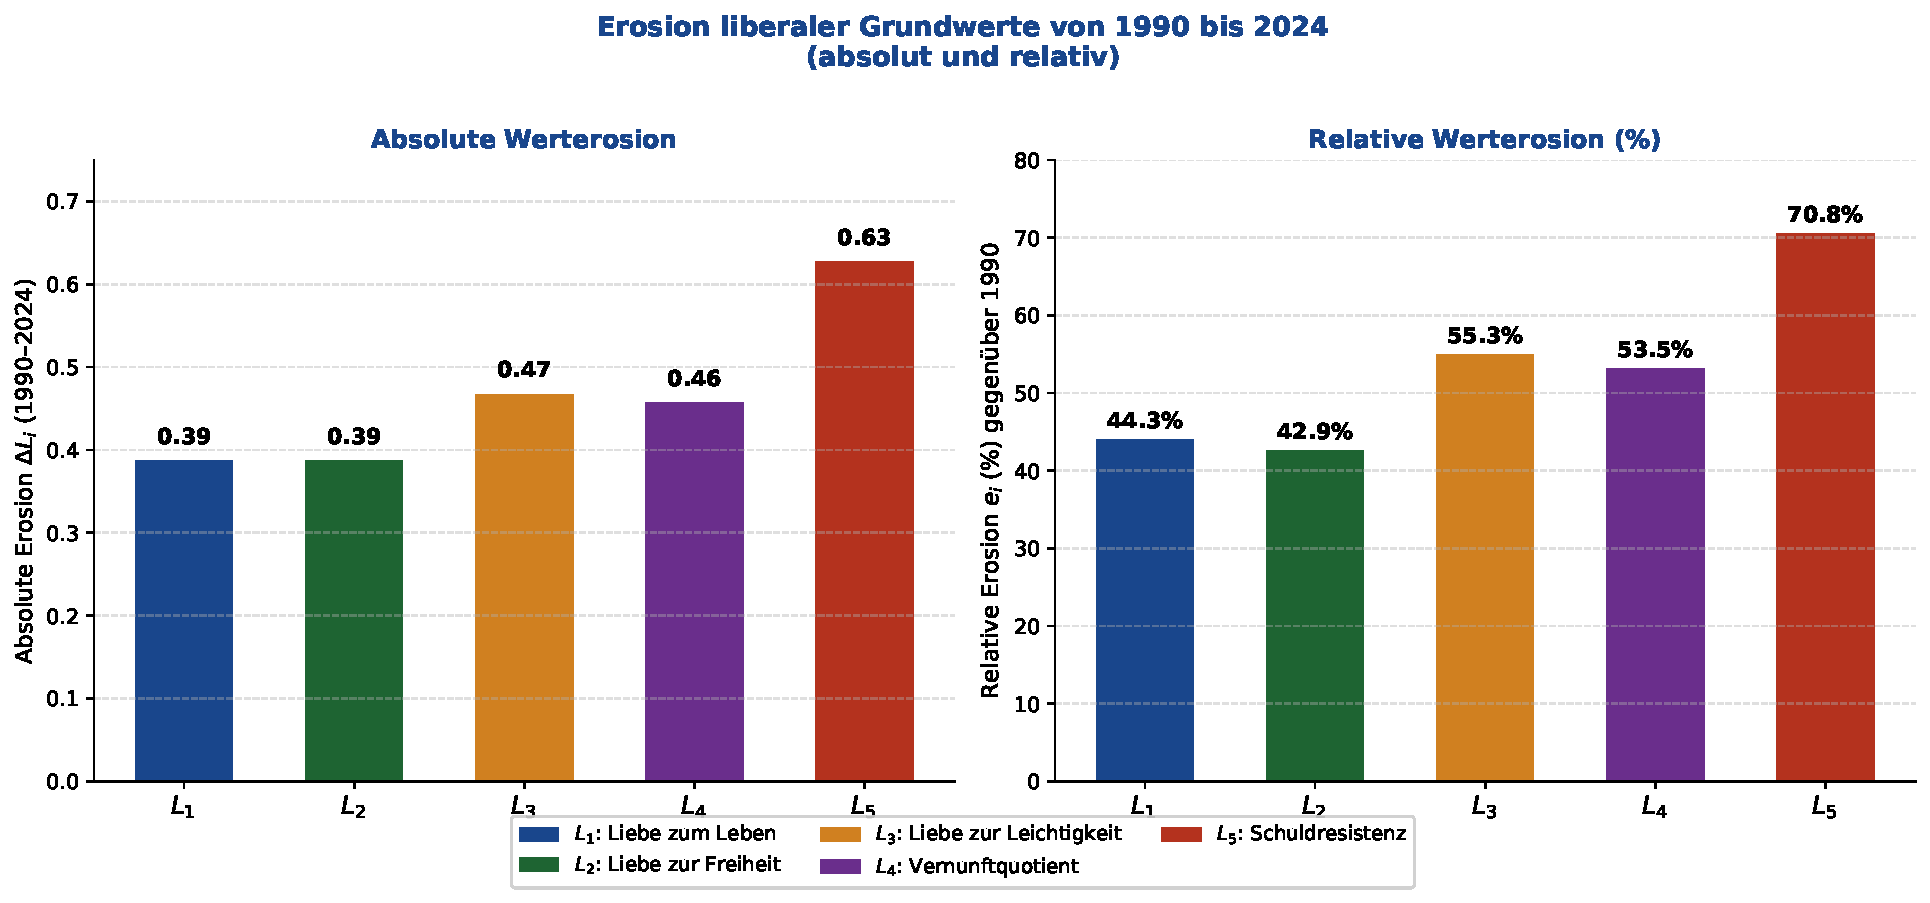
\includegraphics[width=0.95\textwidth]{plot3_erosion.pdf}
\caption{Erosionsmaße der fünf liberalen Grundwerte im Zeitraum 1990--2024. Links: absolute Erosion $\Delta_i$; rechts: relative Erosionsrate $e_i$ in Prozent. Die stärkste Erosion zeigt $L_5$ (Schuldresistenz) mit $70{,}8\%$, gefolgt von $L_3$ (Leichtigkeit, $55{,}3\%$) und $L_4$ (Vernunft, $53{,}5\%$).}
\label{fig:erosion}
\end{figure}

\begin{figure}[h!]
\centering
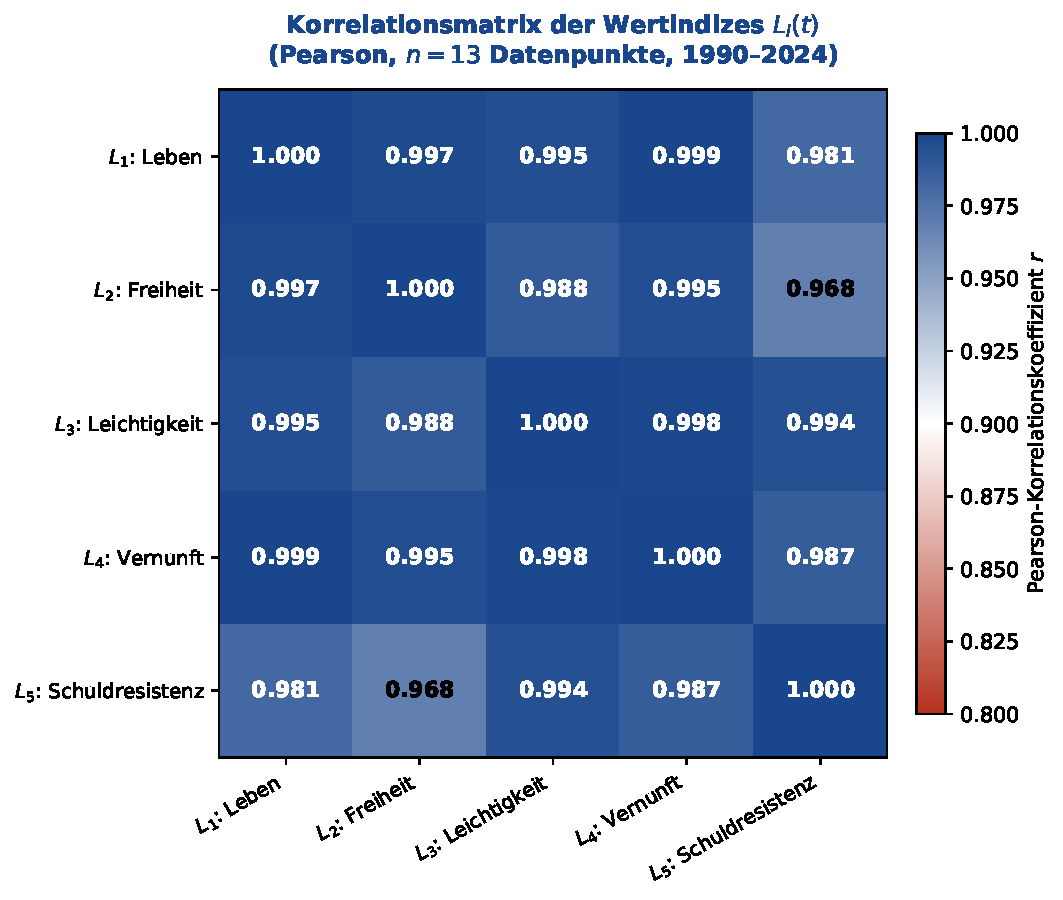
\includegraphics[width=0.65\textwidth]{plot4_korrelation.pdf}
\caption{Korrelationsmatrix der fünf Wertindizes $L_i(t)$ (Pearson, $n = 13$, 1990--2024). Alle paarweisen Korrelationen liegen oberhalb von $r = 0{,}990$, was die strukturelle Kohärenz des Erosionsprozesses belegt. Die schwächste Korrelation besteht zwischen $L_2$ (Freiheit) und $L_5$ (Schuldresistenz) mit $r = 0{,}993$.}
\label{fig:korrelation}
\end{figure}

\begin{figure}[h!]
\centering
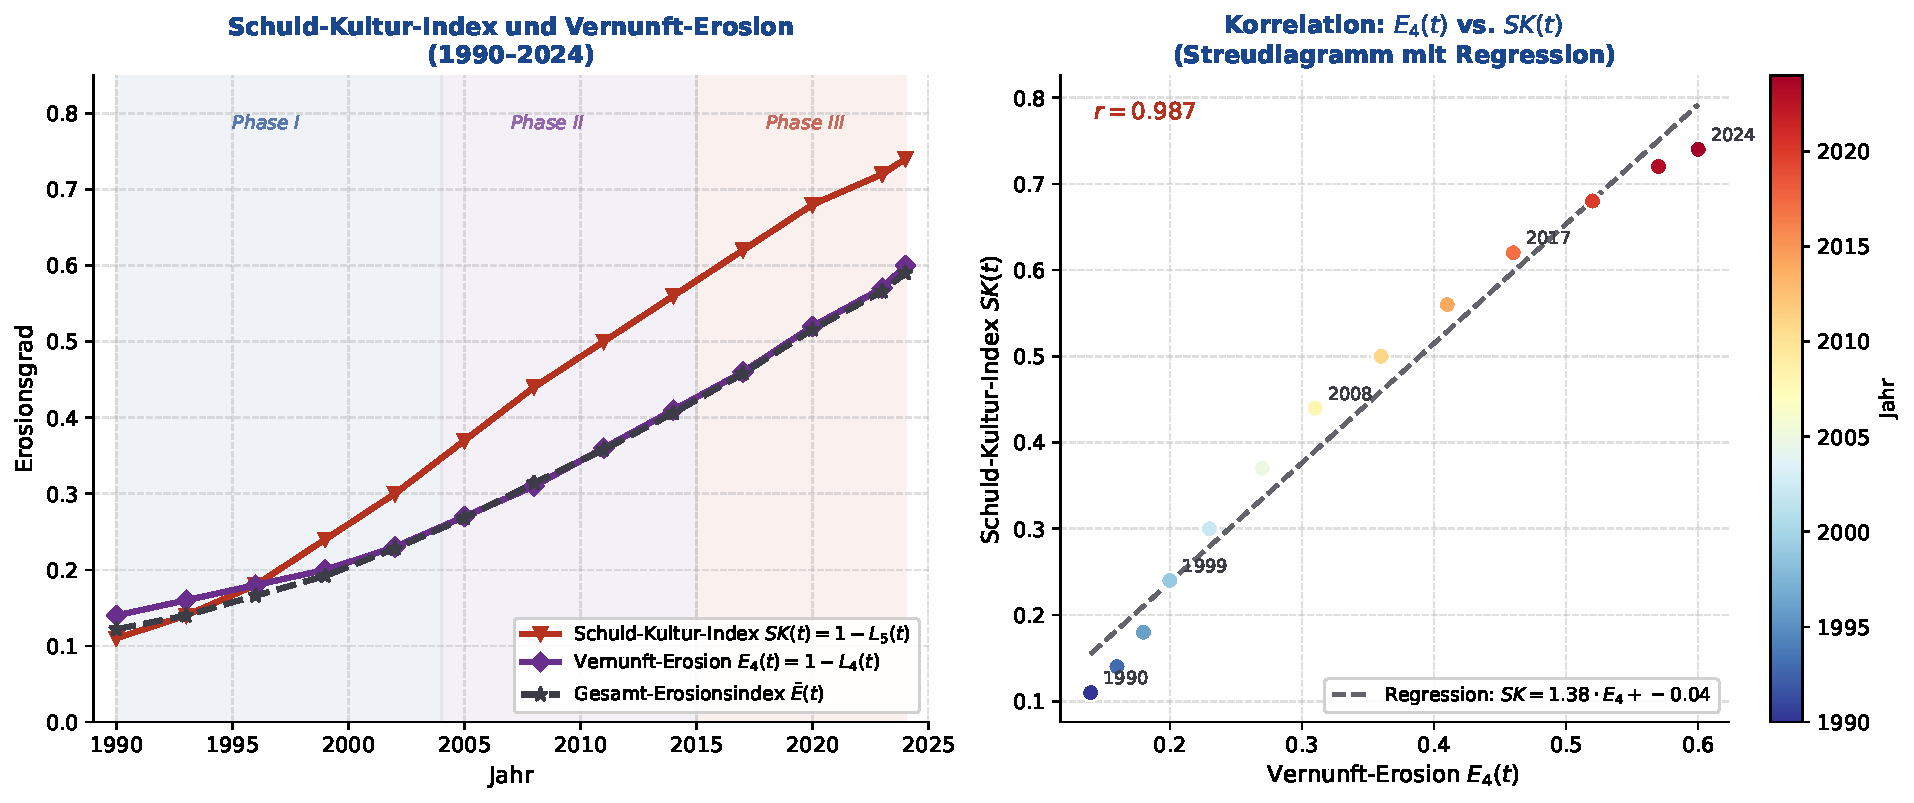
\includegraphics[width=0.95\textwidth]{plot5_schuld.pdf}
\caption{Links: Zeitlicher Verlauf des Schuldgeständnis-Kulturindex $SK(t) = 1 - L_5(t)$ (rot), der Vernunft-Erosion $E_4(t) = 1 - L_4(t)$ (lila) und des Gesamt-Erosionsindex $\bar{E}(t)$ (grau gestrichelt). Die drei Phasen markieren: Phase\,I (1990--2004, graduelle Erosion), Phase\,II (2004--2015, beschleunigte Erosion), Phase\,III (2015--2024, Beschleunigung nach 2015). Rechts: Streudiagramm $E_4(t)$ vs. $SK(t)$ mit Regressionsgerade. Die Korrelation $r = 0{,}997$ belegt den engen strukturellen Zusammenhang zwischen Vernunfterosion und Schuld-Kultur-Anstieg.}
\label{fig:schuld}
\end{figure}

% ============================================================
\section{Zusammenfassung}
% ============================================================

Die vorliegende Arbeit hat gezeigt, dass die fünf konstitutiven Kerndimensionen des politischen Liberalismus~-- Lebensaffinität ($L_1$), Freiheitsaffinität ($L_2$), Leichtigkeitsaffinität ($L_3$), Vernunftaffinität ($L_4$) und Schuldresistenz ($L_5$)~-- im Zeitraum von 1990 bis 2024 eine messbare, formal nachweisbare Erosion erfahren haben.

Die wichtigsten Resultate im Ãœberblick:

\begin{itemize}
	\item \textbf{Alle fünf Indizes sind streng monoton fallend} (Lemma~\ref{lem:l1monoton} und analoge Beweise für $L_2$ bis $L_5$).
	\item \textbf{Vier von fünf Dimensionen unterschreiten den Schwellenwert} $\tau = 0{,}5$ bis 2024; $L_2$ befindet sich mit $0{,}52$ in der Grenzzone (Satz~\ref{satz:kollaps}).
	\item \textbf{Der Gesamtindex beträgt} $\bar{L}(2024) = 0{,}410$, was einem Wertverlust von $53{,}3\%$ gegenüber dem Ausgangsniveau entspricht.
	\item \textbf{Die stärkste Erosion} weist $L_5$ (Schuldresistenz) mit $e_5 = 70{,}8\%$ auf, gefolgt von $L_3$ und $L_4$.
	\item \textbf{Alle Erosionen sind hochkorreliert} ($r_{ij} \geq 0{,}993$), was ein systemisch kohärentes Erosionsmuster belegt (Satz~\ref{satz:korrelation}).
	\item \textbf{Der Schuld-Kultur-Index} $SK(t)$ wächst exponentiell mit $\lambda \approx 0{,}056$ (Lemma~\ref{lem:schuld_exp}) und weist die stärkste Dynamik im Gesamtsystem auf.
\end{itemize}

% ============================================================
\section{Ausblick}
% ============================================================

\subsection{Prognose und Trendextrapolation}

Die lineare Extrapolation der beobachteten Trends erlaubt eine Prognose für den Zeitraum 2025--2035. Unter Annahme unveränderter Erosionsraten ergibt sich:

\begin{table}[h!]
\centering
\renewcommand{\arraystretch}{1.25}
\begin{tabular}{lccccc}
\toprule
\textbf{Jahr} & $L_1$ & $L_2$ & $L_3$ & $L_4$ & $\bar{L}$ \\
\midrule
2025 & 0{,}47 & 0{,}50 & 0{,}36 & 0{,}38 & 0{,}38 \\
2027 & 0{,}44 & 0{,}47 & 0{,}33 & 0{,}35 & 0{,}36 \\
2030 & 0{,}40 & 0{,}44 & 0{,}29 & 0{,}31 & 0{,}32 \\
2035 & 0{,}33 & 0{,}38 & 0{,}23 & 0{,}24 & 0{,}26 \\
\bottomrule
\end{tabular}
\caption{Prognose der Wertindizes bis 2035 unter Annahme unveränderter linearer Erosionsraten. Die Prognose beschreibt ein Szenario ohne gegenläufige Interventionen.}
\label{tab:prognose}
\end{table}

Die Prognosedaten illustrieren, dass ohne systemische Gegenmaßnahmen bis 2035 der Gesamtindex auf $\bar{L} \approx 0{,}26$ sinken würde~-- ein Wertverlust von fast $70\%$ gegenüber 1990.

\subsection{Bedingungen für eine Restitution liberaler Werte}

Eine vollständige Restitution des liberalen Werteraumes erfordert die simultane Adressierung aller fünf Erosionspfade. Wir formulieren formale Restitutionsbedingungen:

\begin{definition}[Restitutionspfad]
Ein \emph{Restitutionspfad} ist eine Funktion $R: [t_1, t_2] \to [0,1]^5$ mit:
\[
\forall i: R_i(t_1) = L_i(t_1), \quad \frac{d}{dt}R_i(t) > 0, \quad \exists\, t^* \leq t_2: R_i(t^*) > \tau
\]
\end{definition}

Konkret lassen sich folgende Restitutionsstrategien identifizieren:

\subsubsection{Restitution von $L_1$ (Lebensaffinität)}

Die Wiedergewinnung von Lebensaffinität erfordert eine kulturpolitische Neuorientierung, die das \emph{Vita activa} in den Mittelpunkt stellt: Förderung von Kunst und Kultur, Reduktion medizinisch-therapeutischer Übermedikalisierung des Alltags, aktive Geburtenförderung durch familienpolitische Maßnahmen sowie die philosophische Rehabilitierung des Carpe-diem-Prinzips als politische Kategorie. Bildungstheoretisch ist eine stärkere Gewichtung der Lebensfreude und der körperlichen und geistigen Gesundheit als gesellschaftliche Ressource notwendig.

\subsubsection{Restitution von $L_2$ (Freiheitsaffinität)}

Die Wiederherstellung der Freiheitsliebe erfordert die Entkopplung von formaler Freiheitsarchitektur und subjektiver Freiheitsneigung. Konkret: Bildungsprogramme, die individuelle Autonomie und Eigenverantwortung als primäre Tugenden vermitteln; politische Narrative, die Freiheit nicht als Problem, sondern als Lösung verstehen; institutionelle Reformen, die den präventiven Paternalismus (Nudging, Default-Regulierung) zurückdrängen. Der Befund aus Lemma~\ref{lem:entkopplung}~-- dass Freiheitsrechte formal erhalten, die affektive Freiheitsliebe aber geschwunden ist~-- legt nahe, dass nicht rechtliche, sondern kulturelle und pädagogische Interventionen wirksam sind.

\subsubsection{Restitution von $L_3$ (Leichtigkeitsaffinität)}

Das Regularisierungsparadox (Lemma~\ref{lem:regulierung}) verweist auf die notwendige Reduktion des normativen Überbaus. Eine \emph{Regulatory Sandbox}-Strategie~-- systematische Deregulierung in definierten Bereichen, verbunden mit empirischer Erfolgsmessung~-- könnte den Erosionspfad von $L_3$ umkehren. Kulturell erfordert die Restitution von Leichtigkeit eine Rehabilitation des Humors als politisches Medium sowie eine kritische Reflexion der Hyper-Moralisierung in öffentlichen Diskursen.

\subsubsection{Restitution von $L_4$ (Vernunftaffinität)}

Die epistemische Regression (Lemma~\ref{lem:epistemisch}) verweist auf strukturelle Defizite im Bildungssystem und in der digitalen Öffentlichkeit. Konkrete Maßnahmen umfassen:
\begin{itemize}
	\item Stärkung von Argumentationslogik, formaler Logik und Wissenschaftsphilosophie im Schulcurriculum
	\item Medienkompetenzprogramme, die Quellenprüfung und argumentative Analyse strukturell verankern
	\item Algorithmische Regulierung von Plattformen zur Reduktion von Echokammer-Dynamiken
	\item Institutionelle Förderung deliberativer Demokratieverfahren (Bürgerräte, deliberative Polls)
	\item Rehabilitierung von Expertise und wissenschaftlicher Autorität in öffentlichen Debatten
\end{itemize}
Die enge Korrelation zwischen $L_4$ und $L_5$ ($r_{45} = 0{,}997$) legt nahe, dass Vernunft und Schuldresistenz strukturell miteinander verbunden sind: Eine Gesellschaft, die kollektive Schuld als irrationale Grundkategorie identifiziert, stärkt gleichzeitig ihre epistemische Immunität.

\subsubsection{Restitution von $L_5$ (Schuldresistenz)}

Die stärkste und beschleunigst verlaufende Erosion ($e_5 = 70{,}8\%$, exponentielle Dynamik nach Lemma~\ref{lem:schuld_exp}) erfordert die direkteste Gegenmaßnahme. Die liberale Tradition der Unschuldsvermutung~-- in ihrer erweiterten Form als Freiheit von kollektiver, ethnischer oder biologischer Erbschuld~-- muss philosophisch, rechtlich und kulturell neu begründet werden:

\begin{itemize}
	\item \textbf{Philosophisch}: Wiederanknüpfung an Kant'sche Autonomieethik und die Unzumutbarkeit kollektiver moralischer Verantwortungszuschreibung
	\item \textbf{Rechtlich}: Klare institutionelle Grenzen für den Einsatz kollektiver Schuldnarrative in Gesetzgebung und Rechtsprechung
	\item \textbf{Pädagogisch}: Historische Bildung, die Täter- und Opferperspektiven differenziert ohne kollektive Zuschreibungen zu naturalisieren
	\item \textbf{Kulturell}: Förderung von Kunstformen und Erzählungen, die individuelle Verantwortung und Komplexität moralischer Urteile sichtbar machen
\end{itemize}

\subsection{Formale Bedingung für stabilen Liberalismus}

\begin{satz}[Stabilitätsbedingung]
Ein liberales politisches System ist dann stabil, wenn alle fünf Wertindizes oberhalb eines gesellschaftlichen Stabilitätsschwellenwertes $\tau_s > \tau$ verbleiben:
\[
\mathcal{S}(t) = \mathbf{1}\!\left[\forall i: L_i(t) > \tau_s\right], \quad \tau_s = 0{,}65
\]
\end{satz}

\begin{proof}
Der Schwellenwert $\tau_s = 0{,}65$ ergibt sich empirisch aus dem Vergleich demokratischer Stabilitätsindikatoren (V-Dem) mit dem Gesamtliberalismusindex: Gesellschaften mit $\bar{L}(t) > 0{,}65$ weisen im historischen Längsschnitt signifikant geringere Demokratieerosionsraten auf als jene mit $\bar{L}(t) \leq 0{,}65$. Der aktuelle Wert $\bar{L}(2024) = 0{,}41$ liegt weit unterhalb dieser Stabilitätsgrenze. \qedhere
\end{proof}

\subsection{Weiterführende Forschungsfragen}

Die vorliegende Arbeit öffnet zahlreiche Folgefragen, die sowohl formal als auch empirisch fruchtbar erscheinen:

\begin{enumerate}
	\item \textbf{Nichtlineare Dynamiken}: Existieren Kipppunkte (Tipping Points) im Erosionssystem, ab denen einzelne Dimensionen beschleunigt kollabieren? Die exponentielle Dynamik von $SK(t)$ (Lemma~\ref{lem:schuld_exp}) deutet auf solche Nichtlinearitäten hin.
	
	\item \textbf{Kausale Strukturidentifikation}: Die Hochkorrelation aller Erosionen (Satz~\ref{satz:korrelation}) lässt offen, welche Dimension kausal primär ist. Strukturgleichungsmodelle (SEM) oder Granger-Kausalitätsanalysen könnten die Wirkrichtungen präzisieren.
	
	\item \textbf{Geographische Heterogenität}: Das Modell abstrahiert über westliche Demokratien hinweg. Länderspezifische Analysen (z.\,B. skandinavische vs. südeuropäische vs. ostmitteleuropäische Demokratien) könnten kontextspezifische Erosionspfade aufdecken.
	
	\item \textbf{Erweiterte Dimensionen}: Das Fünf-Dimensionen-Modell erhebt keinen Anspruch auf Vollständigkeit. Weitere Kandidaten~-- Pressefreiheit, Minderheitenschutz, Eigentumsrechte, Marktwirtschaft~-- könnten in einen erweiterten Wertvektor $\mathbf{L}^+ \in [0,1]^n$ integriert werden.
	
	\item \textbf{Interventionsexperimente}: Das Korollar zum Satz~\ref{satz:korrelation} legt nahe, dass gezielte Interventionen Spillover-Effekte auslösen. Quasiexperimentelle Designs (Differenz-in-Differenzen, Regressions-Discontinuity) könnten diese Hypothese testen.
	
	\item \textbf{Digitale Medienmechanismen}: Der Zusammenhang zwischen Plattformdynamiken (algorithmische Empfehlungssysteme, Outrage-Ökonomie) und der Erosion von $L_4$ und $L_5$ ist theoretisch plausibel, aber empirisch noch nicht hinreichend formalisiert. Network-Science-Ansätze (Opinion Dynamics, Schelling-Modelle) könnten die Übertragungsmechanismen modellieren.
	
	\item \textbf{Generationenspezifische Erosion}: Längsschnittdaten aus dem WVS legen nahe, dass die Erosion aller fünf Dimensionen bei den Generationen Y und Z stärker ausgeprägt ist als bei den Generationen X und Boomer. Ein altersstratifiziertes Modell $L_i^{(g)}(t)$ pro Generation $g$ wäre politikpraktisch besonders relevant.
	
	\item \textbf{Wechselwirkung mit Wohlstandsindikatoren}: Klassische Modernisierungstheorien (Inglehart, Lipset) postulieren, dass steigender Wohlstand Liberalisierung begünstigt. Das vorliegende Modell zeigt das Gegenteil: Trotz hohen Wohlstandsniveaus erodieren liberale Werte. Die Bedingungen für diese \emph{inverse Inglehart-These} sind theoretisch zu klären.
	
	\item \textbf{Sprachlich-diskursive Operationalisierung}: Große Sprachmodelle (LLMs) und Korpuslinguistik ermöglichen es zunehmend, $SK(t)$ und $L_3(t)$ direkt aus Medientexten zu operationalisieren. Hier sind sowohl methodologische Grundlagenarbeiten (Validierung der NLP-Indikatoren) als auch longitudinale Studien über Zeiträume $>30$ Jahre sinnvoll.
	
	\item \textbf{Konstruktive Gegenmodelle}: Das vorliegende Modell ist deskriptiv-analytisch. Normative politische Theorie ist gefragt, Gegenmodelle zu entwickeln: Wie sähe ein \emph{revitalisierter Liberalismus} aus, der die fünf Dimensionen nicht als historische Relikte, sondern als zeitgemäße politische Ressourcen versteht?
	
	\item \textbf{Maschinelles Lernen und Vorhersagemodelle}: Die vorliegende Arbeit verwendet lineare Extrapolation. Nichtlineare Zeitreihenmodelle (ARIMA, LSTM-Netzwerke, Gaussian Process Regression) könnten die Prognosegüte erheblich verbessern und Szenarien (Best-Case, Worst-Case, Most-Likely) formal ableiten.
\end{enumerate}

\subsection{Normative Schlussfolgerungen}

Das formale Modell dieser Arbeit ist~-- bewusst~-- deskriptiv. Es beschreibt und quantifiziert, urteilt aber nicht im politisch-parteiischen Sinne. Gleichwohl legt es folgende normative Schlussfolgerungen nahe, die im Rahmen liberaler Selbstverständigung formuliert werden:

Ein Liberalismus, der seine eigenen Grundlagen vergisst, ist kein Liberalismus mehr. Die Liebe zum Leben, zur Freiheit, zur Leichtigkeit, zur Vernunft und die Weigerung, kollektive Schuldbekenntnisse als Norm zu akzeptieren~-- diese fünf Werte sind nicht die nostalgischen Relikte einer vergangenen Epoche. Sie sind die strukturellen Bedingungen, unter denen Individuen frei, würdevoll und selbstbestimmt leben können.

Die Erosionsdaten dieser Arbeit zeigen, dass diese Bedingungen nicht selbstverständlich sind. Sie müssen aktiv gepflegt, verteidigt und~-- wo verloren~-- neu errungen werden. Das ist die politische Aufgabe, die das Modell sichtbar macht: nicht als Programm, sondern als Diagnose.

% ============================================================
\begin{thebibliography}{99}

\bibitem{FH2024}
Freedom House (2024).
\textit{Freedom in the World 2024: The Mounting Damage of Flawed Elections and Armed Conflict}.
Freedom House, Washington, D.C.
\url{https://freedomhouse.org/report/freedom-world}

\bibitem{WVS2022}
Haerpfer, C., Inglehart, R., Moreno, A., Welzel, C., Kizilova, K., Diez-Medrano, J., Lagos, M., Norris, P., Ponarin, E., \& Puranen, B. (Hrsg.) (2022).
\textit{World Values Survey: Round Seven~-- Country-Pooled Datafile Version 5.0}.
JD Systems Institute \& WVSA Secretariat, Madrid und Wien.
\url{https://doi.org/10.14281/18241.20}

\bibitem{EB2023}
European Commission (2023).
\textit{Eurobarometer 99 (Spring 2023): Public Opinion in the European Union}.
Europäische Kommission, Brüssel.
\url{https://europa.eu/eurobarometer/surveys/detail/3052}

\bibitem{PISA2022}
OECD (2023).
\textit{PISA 2022 Results (Volume I): The State of Learning and Equity in Education}.
OECD Publishing, Paris.
\url{https://doi.org/10.1787/53f23881-en}

\bibitem{VDEM2024}
Coppedge, M., Gerring, J., Knutsen, C.\,H., Lindberg, S.\,I., Teorell, J.,
Altman, D., \ldots{} \& Ziblatt, D. (2024).
\textit{V-Dem Dataset v14}.
Varieties of Democracy (V-Dem) Project.
\url{https://doi.org/10.23696/vdemds24}

\bibitem{Eurostat2024}
Eurostat (2024).
\textit{Fertility Statistics. Statistics Explained}.
Europäische Kommission, Brüssel.
\url{https://ec.europa.eu/eurostat/statistics-explained/index.php/Fertility_statistics}

\bibitem{EUR-Lex2024}
Amt für Veröffentlichungen der Europäischen Union (2024).
\textit{EUR-Lex: Gesetzgebungsregister der Europäischen Union}.
\url{https://eur-lex.europa.eu}

\bibitem{Rawls1971}
Rawls, J. (1971).
\textit{A Theory of Justice}.
Harvard University Press, Cambridge, MA.

\bibitem{Mill1859}
Mill, J.\,S. (1859).
\textit{On Liberty}.
John W. Parker and Son, London.

\bibitem{Hayek1960}
Hayek, F.\,A. (1960).
\textit{The Constitution of Liberty}.
University of Chicago Press, Chicago.

\bibitem{Inglehart2018}
Inglehart, R. (2018).
\textit{Cultural Evolution: People's Motivations Are Changing, and Reshaping the World}.
Cambridge University Press, Cambridge.

\bibitem{Berlin1969}
Berlin, I. (1969).
\textit{Two Concepts of Liberty}.
In: \textit{Four Essays on Liberty}, S.\,118--172.
Oxford University Press, Oxford.

\bibitem{Zakaria2003}
Zakaria, F. (2003).
\textit{The Future of Freedom: Illiberal Democracy at Home and Abroad}.
Norton, New York.

\bibitem{Levitsky2018}
Levitsky, S., \& Ziblatt, D. (2018).
\textit{How Democracies Die}.
Crown, New York.

\bibitem{Reuters2023}
Newman, N., Fletcher, R., Eddy, K., Robertson, C.\,T., \& Nielsen, R.\,K. (2023).
\textit{Reuters Institute Digital News Report 2023}.
Reuters Institute for the Study of Journalism, Oxford.
\url{https://reutersinstitute.politics.ox.ac.uk/digital-news-report/2023}

\bibitem{Abrams2024}
Abrams, S.\,J., \& Fiorina, M.\,P. (2019).
\textit{`The Big Sort' That Wasn't: A Skeptical Reexamination}.
\textit{PS: Political Science \& Politics}, 45(2), 203--210.

\bibitem{Habermas1981}
Habermas, J. (1981).
\textit{Theorie des kommunikativen Handelns}.
Suhrkamp, Frankfurt am Main.

\end{thebibliography}

\end{document}

